% delete the .aux file if "!Package babel Error: You haven't defined the language ENGLISH yet."
\documentclass[aip,jcp,numerical,reprint]{revtex4-1}
\usepackage{graphicx}  % needed for figures
\usepackage{threeparttable} % for annotated table
\usepackage{siunitx} % for decimal alignment in tables
\usepackage{bm,amssymb,amsmath} % for math
\usepackage[bookmarks]{hyperref} % for reference links
\usepackage[svgnames]{xcolor} % to define color names
\definecolor{Blue}{RGB}{0 0 128}
\hypersetup{ %options-for-appearance-of-links-in-hyperref
	colorlinks= true,
    allcolors = Blue
}
\usepackage{tikz}
\usetikzlibrary{calc} % for tikz calculations
\usetikzlibrary{arrows,decorations.markings} % make arrow head bigger
\usepackage{color,soul} % for reviews

\usepackage{comment}
\begin{document}

\title{Interpolated wave functions for nonadiabatic simulations with the fixed-node quantum Monte Carlo method}
\author{NMT, YY, SHS, DMC}
\affiliation{Department of Physics, University of Illinois, Urbana, Illinois 61801 USA}

\begin{abstract}
Simulating nonadiabatic effects with many-body wave function approaches is an open field with many challenges.  %Various algorithms can be applied that capture the phenomenology of nonadiabatic effects beyond the Born-Oppenheimer approximation, however except in very few cases its hard to determine how accurate such calculations are.
Recent interest has been driven by new algorithmic developments and improved theoretical understanding of properties unique to electron-ion wave functions.  Fixed-node diffusion Monte Caro is one technique that has shown promising results that is potentially scalable to larger systems.
%This has come in several different forms, which include studies that focus on the form of the wave function, highly approximate methods that focus on correlations between electrons and ions, and more exact methods that work for model Hamiltonians or small systems, which includes density matrix renomarlization group, quantum monte Carlo, explictly correlated gaussians, as well as some analytically exact results.  
%Here we briefly review different theoretical approaches to  treating quantum simulations beyond the Born-Oppenheimer approximation, with a focus on quantum Monte Carlo result.  
In particular we focus on the CH molecule for which previous results showed a large contribution to the energy from nonadiabatic effects.  We suggest a new wave function ansatz for diatomic systems which involves interpolating the determinant coefficients calculated from configuration interaction methods.    We find this to be an improvement on previous wave functions forms that have been considered.    The amount of nonadiabatic energy in the CH molecule is reduced from previous results, but still remains the largest among the molecules under consideration.

\end{abstract}
\maketitle

\section{Introduction}
The Born-Oppenheimer approximation is considered to be one of the most accurate approximations used in the simulation of chemical and condensed matter systems~\cite{Tubman_ECG,Martinez_Review,Cederbaum_Review}.     However, the breakdown of the Born-Oppenheimer approximation can lead to interesting new physics and in some cases even giant effects~\cite{saitta2008,giustino2016}. The full impact of using the Born-Oppenheimer approximation is still not widely understood due to the lack of theoretical methods that can go beyond the Born-Oppenheimer approximation accurately, although there has been significant progress recently made in this direction\cite{Tubman_ECG,Yang2015,Sharon_NEO-HF,Sharon_XCNEO-HF1,Sharon_XCNEO-HF2,Sharon_XCNEO-HF,Kurt_XCNEO-HF,Kurt_XCNEO-HF1,Sharon_NEO-DFT,Sharon_NEO-DFT2,Sharon_NEO-DFT3,Gross_NEO-DFT,Gross_NEO-DFT1,Ilkka_Path,Ilkka_Path1,Ilkka_Path2}.  While nonadiabatic effects are generally ignored in many applications, there are several important places where highly accurate simulations that go beyond the Born-Oppenheimer approximation is imperative.  For example, the identifications of molecules in the diffuse interstellar bands (DIB) is one such case where highly accurate energies without the Born-Oppenheimer approximation is needed of both ground and excited states~\cite{snow2006}.   There has been much interest in recent experiments have been able to identify several peaks that correspond to ionized C60 in the DIB\cite{campbell2015}.  However, many molecule remain unidentified and as such there are still many open questions as to the physical processes that occur in the interstellar medium.   Theoretical approaches have not been widely used to directly identify absorption lines in the spectrum due to a lack of accuracy in current simulations.  

While identifying absorption peaks in the DIB is beyond what we can simulate currently, we have started developing quantum Monte Carlo techniques to make progress in this direction\cite{Tubman_ECG,Yang2015}.   Our current focus has been to benchmark molecular systems in which the interactions between the electrons and ions are not approximated.   Fixed-node diffusion Monte Carlo (FN-DMC) is a method in which results are only biased by what is called the fixed-node approximation.  %This is an approximation that is based on a trial wave function, for which only the nodes (where the amplitude of the wave function goes to zero) determine the quality of the result.  Thus is the nodes of a trial wave function is exact, the resulting energies will be unbiased.  Also the fixed-node approximation is a variational approximation, thus the better the nodes the lower the energy.  
The fixed-node approximation has been tested extensively and is among the best algorithms for clamped-ion simulations~\cite{grossman1,Tubman_Release,Tubman_ACS}.  In the case of simulations that go beyond the Born-Oppenheimer approximation, recent benchmarks demonstrated some of the most accurate energies ever calculated for a series atomic and diatomic systems~\cite{Yang2015}.

There is however much development still needed to improve the accuracy and scalability of these simulations even further.  The nonadiabatic effects in the atomic and and diatomic systems, as calculated from FN-DMC simulations,  were generally smaller than 0.1~mHa. There were two exceptions to this; the BH and CH molecules. In particular the CH molecule had an unexpectedly large contribution to the nonadiabatic energy.   While it is likely that there is some nonadiabatic effects in the CH molecule, it is hard to determine exactly how much due to the fixed-node error.   To address this question further, in this work we use an improved wave function ansatz over the previous simulations on CH.
%In this work we review progress we have made in improving the accuracy of  ground state of calculations beyond the Born-Oppenheimer approximation, and we demonstrate a new wave function ansatz that is more accurate than in previous work.


\section{Fixed-Node Diffusion Monte Carlo (FN-DMC)}
Diffusion Monte Carlo~\cite{Anderson_DMC,lester1,Stuart_Review,Needs_Review,Needs_Old_Review,QMC_Review} is a projector method that evolves a trial wave function in imaginary time and projects out the ground-state wave function. For practical simulations of fermions, the fixed-node approximation is introduced, which depends only on the set of electronic positions where a trial wave function is equal to zero.  %A wave function that jointly describes electrons and ions simultaneously is something that is not limited to nonadiabatic simulations.    Very specific wave functions forms are used to calculate harmonic and anharmonic effects within the Born-Oppenheimer approximation.  
  Wave function forms that go beyond the Born-Oppenheimer approximation are not hard to generate, but finding accurate forms is an open question that has generated  much recent interest~\cite{cederbaum1,cederbaum12,Tubman_ECG,boent,gross2014}.  For the diffusion Monte Carlo method the treatment of electron-ion wave functions requires minimal changes.  The main differences are seen in evaluating a different form of the trial wave function, and  evaluating the kinetic energy term for the nuclei.   This nodal surfaces  depends on the coordinates of both the electrons and ions simultaneously, which is different from other methods that can simulate Hamiltonians beyond the Born-Oppenheimer approximation\cite{mitroy2013,Kurt_XCNEO-HF,Sharon_NEO-DFT,kerley2013}.% and we have recently shown that we can generate high-quality nodal surfaces for a range of systems that include full electron-ion wave functions. 

For clamped-ion simulations, the fixed-node approximation has been tested extensively with many different types of wave functions.  When the trial wave function has the same nodal surface as the exact ground-state wave function, FN-DMC yields the unbiased ground-state energy.  Approximate nodal surfaces can be generated through wave function optimization.  Approximate nodal surfaces have been tested on a wide range of systems and provide results comparable to the state of the art in \textit{ab initio} simulations.~\cite{Stuart_Review,rothstein1,grossman1,Yang2015,Tubman_Release} In addition, the energies generated with FN-DMC are variational with respect to the ground-state energy.


With the exception of some very recent research, there has been little work in treating nonadiabatic simulations of ground state wave functions with FN-DMC~\cite{Tubman_ECG,Yang2015}.  One of the most well known studies is by Chen and Anderson   on  the H$_{2}$ molecule~\cite{chen1995}.  The wave function in this work is specified completely in terms of relative coordinates and only a few variational parameters.  
%This wave function is a product of four terms, two of which are electronic orbital that consists of a sum of two exponentials.  The  other two terms are Jastrow terms for the electron-ion and electron-electron correlations, which captures all the wave function cusps.  
Since all terms used in the wave function depend only on relative distances and are rotationally symmetric, the ions and electrons are free to rotate and translate in space.   This type of wave function is different from the typical single particle basis sets that most quantum chemistry methods use, and is related to the correlated wave function approaches used in the Hylleraas and explicitly correlated gaussian (ECG) approach.  

The success of H$_{2}$ is misleading because it can always be simulated exactly with diffusion Monte Carlo, as it has no sign problem~\cite{Tubman_Release}.  This implies that there are no systematic biases in the DMC simulation, and thus the best DMC results can be considered those that have the smallest error bar.  Therefore the variance of the local energy and the computational expense needed to evaluate the trial wave function are the important factors for generating a wave function to simulate H$_{2}$.  For most other systems, the fixed-node approximation has to be employed, and then the quality of the nodal surface becomes a crucial aspect that determines the accuracy of a simulation.  Thus the challenge of performing FN-DMC on such systems is to find good wave function forms that generate nodal surfaces of high quality.
%The Chen-Anderson energy for the H$_{2}$ molecule has an the error bar slightly smaller than 10$^{-5}$ (a.u.).  While this a highly accurate result, there are several other non-QMC results, including one by Bubin-Adomwicz, that are thought to be accurate to many more digits, even though there is some inherent bias due to a finite basis set.  The Bubin-Adomwicz result uses a basis of explicitly correlated gaussian which produces many terms that require an exponential amount of computational cost with increasing system size. 
%In larger systems, it is in many cases too expensive to converge the wave functions, with either method, to such high accuracy.  In FN-DMC there is an error associated with treating fermions, and with the ECG technique, the computational cost grows too quickly to converge the wave function, For large systems, full CI would also become prohibitively expensive.  

%For static ion simulations, FN-DMC  it is a highly accurate technique, even for large systems despite the fixed-node approximation.  The question becomes how to create a trial wave function to use in FN-DMC for electron-ion methods.
%Using recent improvements in generating highly accurate wave functions that can be optimized with FN-DMC, we have shown in previous work that highly accurate wave functions can be generated for electron-ion systems.  However, for applications of spectroscopy, it remains an open question if we can push our simulations to be accurate enough to solve questions related to identifying ISM peaks for instance.


\subsection{Electron-Ion Wave Function}
 There are several forms in which one might try to build a wave function for electron-ion systems.  The previously discussed wave functions used for H$_{2}$ are not easy to scale up to larger systems in which defects in the nodal surface can cause biases in the final results.   %Other than the type of wave function used in Chen-Anderson, the other well known wave function for electron-ion systems is a single determinant of plane waves for both the electrons and ions, which doesn't change as the ions move.  The cusps are enforced by a Jastrow, which does move with the electron and ions, but the accuracy of the calculations are limited by the nodes, which as plane waves, do not spend on the physical interactions between the electrons and ions.  
%We expect the best wave functions that one can use for these calculations is a full position dependent electronic wave function, that is optimized at each ionic position.  Ideally one would like to optimize all wave function parameters at each ion position.  For many ion problems, this would require each walker to have its own wave function and because of the stochastic nature of optimizing wave functions, the wave function is not guaranteed to be consistent as the ions move around.  Static Jastrow parameters have been used in CEIMC type calculations, which would alleviate that problem, however a wave function call would have to be made to an external program for each walker for each  ion configuration, which is more computationally expensive and technically difficult than should be considered for our first electron-ion wave functions.   
In previous work we have considered several different wave function forms that make use of standard clamped-ion quantum chemistry methods~\cite{Tubman_ECG}. %in order create wave functions for nonadiabatic FN-DMC calculations. 
%Before discussing the form considered in this work, we note that there are many possibilities for creating such wave functions for use in QMC, and there is certainly room for a l significant development in this direction.  
We considered three classes of wave functions that are progressively more accurate as follows:
\begin{align}
\Psi(r,R) =& e^{J(r,R)}\phi(R)\sum_{i}\alpha^{*}_{i} D_{i}(r) \label{eqn:wfs1}\\
\Psi(r,R) =&e^{J(r,R)}\phi(R)\sum_{i}\alpha^{*}_{i} D_{i}(r,R^{*}) \label{eqn:wfs2}\\
\Psi(r,R) =& e^{J(r,R)}\phi(R)\sum_{i}\alpha^{}_{i}(R) D_{i}(r,R), \label{eqn:wfs3}
\end{align}
where $r$ refers to the coordinates of all the electrons and $R$ to those of all the ions.  $J(r,R)$ is the Jastrow term which involves variational parameters that correlate the quantum particles and additionally  enforce cusp conditions in the wave function.  $\phi(R)$ is the nuclear part of the wave function. The final terms correspond to determinants $D$ and the corresponding coefficients $\alpha$.    The $*$ denotes how these terms are evaluated, as will be discussed. 

The nuclear part of the wave function is chosen to be a simple product of gaussian functions over each nucleus pair: 
\begin{align}
%\phi(R) \propto \prod_{\substack{i \\ i<j}} \exp\left[-a_{ij}\left(|R_{i}-R_{j}|-b_{ij}\right)^2\right], 
\phi(R) \propto \prod_{\substack{i \\ i<j}} e^{-a_{ij}\left(|R_{i}-R_{j}|-b_{ij}\right)^2}, 
\end{align}
where $a$ and $b$ are optimizeable parameters. In our calculations $a_{ij}$ has only a single optimized value $a$, and for $b_{ij}$ we use the Born-Oppenheimer equilibrium distance between the species involved.

The terms in these wave functions involve very specific calculations that are performed and optimized in both quantum chemistry codes and quantum Monte Carlo codes.  
%The differences between the wave functions is in how we  compute the determinant of the electrons $D_{i}$.  
The determinant terms, $\alpha_{i}^{*}D_{i}(r) $, $\alpha_{i}^{*}D_{i}(r,R^{*}) $, and $\alpha_{i}^{}D_{i}(r,R)$ differ based on how we optimize the determinant coefficients $\alpha$ and how we parameterize the evaluation of the determinants based on the ion coordinates $R$.   

The  wave function in Eq.~\eqref{eqn:wfs1} is the least accurate of the three wave functions and has a fixed determinant regardless of where the ions are.  The term $\alpha^{*}$ indicates that the determinant coefficients have been optimized at the equilibrium geometry.  
%Practically this is implemented by having the determinant part of the wave function independent of the ion positions.  
Both the ionic part of the wave function ($\phi$) and the Jastrow depend on the ion positions, which is important as the Jastrow maintains the cusps between all the quantum particles.  

%This form of the wave function has previously been used for large-scale simulations of metallic hydrogen~\cite{ceperley3,natoli1,natoli2}.  %As an ansatz the wave function in this work  used a single determinant of plane waves for both the electrons and ions, with only the electron-ion Jastrow to capture the interactions between the two species.  
The problem with this type of wave function is that the accuracy is limited by the electronic nodes, which do not depend on the ion positions.
%This may be a good approximation for condensed matter systems, but in general  the determinant should depend on the ionic coordinates. 
%This is especially important for heavier atoms, beyond helium, in which the core orbitals should track the ion positions. 
The wave function in Eq.~\eqref{eqn:wfs2} fixes this problem.  
%is improved over the previous wave function in that the nodes of the determinant part of the wave function depend on the ion positions.  
The $\alpha^{*}$ indicates that the determinant part of the wave function is optimized for the equilibrium ion positions, as in the previous wave function, but the term $R^{*}$ signifies that the determinant  depends on the position of the ions through the basis set.  Basis sets in molecular calculations are generally constructed from local orbitals centered around the atoms.  In these calculations a single particle orbital is written as $\theta(r) = \sum_{ji}\gamma_{j}(r-R_{i})$, where \textit{i} is an index for an ionic center, and \textit{j} is an index for a basis set element.  
In this form, wave functions depending on the ion positions are straightforward to create and optimize,
%Wave functions in this form provide a straightforward way  of creating and optimizing wave functions that depend on the ion positions.  
%For systems that are not strongly nonadiabatic, the wave function will not significantly change depending on the ion positions, and thus this wave function ansatz should be good, especially for describing the electronic nodes.
%  There are some problems with this form of the wave function, as for instance single particle orbitals can have directional dependence, such as in a covalent bond.  
but difficulties may arise with the possible directional dependence of the single body orbitals, such as in covalent bonds. %This can be addressed with directionally dependent Jastrows, but we go further than this, as will be discussed.  
%This form of the wave function is similar to the wave function used in Ref.~\cite{ceperley3} for the molecular hydrogen phases.   They are not quite the same, however, as the electronic orbitals and ionic orbitals were centered around fixed positions and thus the electronic orbitals did not explicitly track the ion positions.   A few of the simulations did have the electrons track the centers of the hydrogen molecules as they changed position.

Eq.~\eqref{eqn:wfs3} represents what we expect to be the best wave function considered here, since it has explicit dependence on the ion positions for the single particle orbitals and the determinant coefficients. Essentially this amounts to recalculating a wave function from scratch each time the ion positions are changed.  In practice this would significantly increase the computational cost of these simulations as well as cause many technical challenges.  The main focus of this current work is to describe a technique in which this can be done efficiently for diatomic systems. 
% Ideally one would like to optimize all wave function parameters at each ion position.  
%One way to implement this would be to assign each walker its own separate wave function. Because of the stochastic nature of optimizing wave functions, it is possible that a wave function may not be entirely single valued as the ions move around.  Static Jastrow parameters have been used in coupled electron ion Monte Carlo calculations, which would alleviate this problem; however a wave function call would still have to be made to an external program for each walker and for each ion configuration.  

%Equation \ref{eqn:wfs3}, is a very accurate form of the wave function in which all variational parameters, except those in $\phi$, are full optimized at all ion positions.  This is a very expensive form of the wave function to maintain, and its not entirely clear in its most flexible form how to make it completely consistent, since the wave functions parameters are stochastically optimized.  Additionally this form requires each walker to have its own wave function, which can be technically challenging during a FN-DMC run.  Thus we focus on wave function in equation \ref{eqn:wfs2} in this work.

\section{Dragged Node Approximation}


The fixed-node approximation is generally going to result in errors in the energy that overestimate the nonadiabatic effects.   This is a result of the increased complexity of optimizing wave functions for the full electron-ion system.   When the fixed-nuclei energies are more accurate than the electron-ion wave functions, then we will see an overestimate of the nonadiabatic energy.   %This is to say that the energy difference between the the fixed-nuclei simulations and the dynamic simulation will be overestimated.
  It should be noted that this expectation isn't always true, as seen in previous benchmarks comparisons of (Be,Be+,B,B+,C+) in comparison to highly converged ECG results~\cite{Yang2015}.  While it does appear that in some cases the nonadiabatic simulations are as good or more accurate than our clamped-ion simulations, this is less likely for molecular systems in which the ions can move relative to each other.    %Regardless, when large nonadiabatic effects are soon, it is important to consider how big the fixed-node approximation really is.  

Recent simulations with quantum Monte Carlo have have used a particular type of nodal structure which is called the  dragged-node approximation~\cite{Tubman_ECG,Yang2015}.
%To understand the dragged-node approximation  it is important to consider the different nodal structures in the wave functions given by Eqs.~\eqref{eqn:wfs2} and \eqref{eqn:wfs3}.  In Eq.~\eqref{eqn:wfs3}, the nodes are defined by the determinant that is calculated at each position in space, but 
This approximation can be used for wave functions in the form of Eq.~\eqref{eqn:wfs2} in which  we generate a wave function from the electronic nodes defined at the equilibrium geometry.   When the ions change position the wave function changes based on the basis set dependence of the ion coordinates. The change in the wave function causes a corresponding change in the nodes.  
 The dragged-node approximation is completely variational when used in FN-DMC.  
For systems that do not show strong nonadiabatic behavior, we expect this to be an excellent approximation. %as this works best when the nodes of a wave function does not change sharply as the ions change positions. 
 Thus it was surprising that the energy due to nonadiabatic effects in a previous calculation of the CH molecule~\cite{Yang2015} was larger than expected.   To test the validity of this result we wanted to improve upon the wave function used in this previous work.%    In this work we exploit that the CH molecule is made up for only two atoms, and create a wave function of type Eq.~\eqref{eqn:wfs3} that is computationally feasible to calculate.   A wave function of this type can have significantly more complicated dependence of the nodes based on the ion positions than used in the dragged-node approximation.

\section{Improving wave functions}

%To understand how strong the nonadiabatic effects are in CH, we wanted to consider a wave function in which there were more variational degrees of freedom for the nodes.  As described previously, 
The wave function in Eq.~\eqref{eqn:wfs3} is much more general than what we included in our previous studies, but is harder to generate.  In general it is not feasible to do a full wave function evaluation for each new configuration of the ions.  However, for diatomic molecules it is feasible to precompute and optimize wave functions at different distances and then use the precomputed calculations in order to interpolate some of the  wave function parameters.  There are several different ways this can be done.   The first wave function one might consider is to use a grid with respect to the distance between the ions, and calculate a fully optimized electronic wave function at each grid point.  With this form it is possible to evaluate the electronic wave function at each grid point and use an interpolation scheme to determine the actual electronic wave function given a distance between the ions.  This would be multiplied by a purely ionic wave function, as in Eq.~\eqref{eqn:wfs3}. Although this is technically a feasible way to generate improved wave functions,  we found that this approach was difficult to implement with regards maintaining a smooth wave function.   

A second approach, for which we present results in this work, uses determinant coefficients as a function of the ion positions.  For a diatomic system, this corresponds to generating a 1D function for each determinant coefficient.  This is an improvement over the dragged-node approximation, as the coefficients of the determinants are allowed to change with ion distance, and can capture complicated ion dependences of the nodes.  In future work it also might be possible to extend this type of wave function to at least three particles, which would require fitting functions for the determinant coefficients in higher dimensions.  





% As a large distance,  but still in the region in which the ions sample, we optimize an electronic wave function, but only the determinant coefficients.  We fix the Jastrow to be the same as the one we optimized at the equilibrium position.  We then take all the determinant coefficients for the two different wave functions, and fix a second order polynomial to them (there are general a few hundred of these), for which we then use to interpolate the multi-determinant wave function for all ion positions.  

\section{ Wave function details}
%There are several different approaches for generating electronic wave functions for a FN-DMC calculation.~\cite{Umrigar_Alleviation,Toulouse_Bench,Brown_Bench,Seth_Bench} Recent advances~\cite{Nightingale_Linear,Umrigar_Linear,Brown_Bench} have made it possible to simultaneously optimize thousands of wave function parameters using variational Monte Carlo with clamped-ions. 
We compare two types of wave functions in this work, one of form given by Eq.~(\ref{eqn:wfs2}) and one of form given by  Eq.~(\ref{eqn:wfs3}).  For the first form, we use an initial guess for the wave function that is generated from complete active space self-consistent-field (CASSCF)~\cite{Chaban_MCSCF,Szabo} calculations using the quantum chemistry package GAMESS-US.~\cite{GAMESS} The optimized orbitals are then used in a configuration interaction singles and doubles (CISD) calculation to generate a series of configuration state functions (CSFs).~\cite{Pauncz_CSF} For the small systems LiH and BeH, a CASSCF calculation with a large active space is used in place of CISD. The multi-CSF expansion of the wave function can be expressed in the following form,
\begin{align}
\Psi_{\text{CISD}}(\vec{r};\vec{R}_o)=\sum\limits_{i=1}^{N_{\text{CSF}}}c_i\phi_i(\vec{r};\vec{R}_o), \label{eq:psi_gms}
\end{align}
where $\vec{r}$ refers to the spatial coordinates of all the electrons and $\vec{R}_o$ refers to the equilibrium positions of all the ions. $\phi_i(\vec{r})$ and $\vec{\alpha}=\{\alpha_1,\alpha_2,\dots\}$ are the CSF coefficients generated from CISD. The cc-pV5Z basis~\cite{dunning} is used for the atomic systems and the Roos Augmented Triple Zeta ANO basis~\cite{roos} is used for the molecular systems except for the smallest system LiH, where the cc-pV5Z basis is used.

After the multi-CSF expansion is generated, we impose the electron-nucleus cusp condition on each molecular orbital~\cite{cusp} and add a Jastrow factor to the wave function to include electron correlation.~\cite{Kato} Our Jastrow factor contains electron-electron, electron-nucleus and electron-electron-nucleus terms. The full electronic wave function used in FN-DMC is,
\begin{align}
\psi_e(\vec{r};\vec{R})=e^{J(\vec{r},\vec{R},\vec{\beta})}\Psi_{\text{CISD}}(\vec{r};\vec{R})\label{eq:psie}.
\end{align}
We optimize the CSF and Jastrow coefficients, $\vec{\alpha}$ and $\vec{\beta}$, respectively, simultaneously with QMCPACK.~\cite{QMCPACK_Kim,QMCPACK_Esler} Optimization is performed with the ions clamped to their equilibrium positions. The equilibrium geometries for BeH and BH are chosen to be the ECG-optimized distances for comparison with the ECG  method, and the geometries for the rest of the hydrides are taken from experimental data.~\cite{CCCBDB}

For the second type of wave function, we consider a form of type Eq.~(\ref{eqn:wfs3}) for the CH molecules.  This involves the following additional steps. At the equilibrium C-H separation $R_e=2.1165$ bohr, optimize the electronic wave function, which includes all determinant coefficients and a Jastrow. At two C-H separations near equilibrium $R_{\text{left}}=2.0$ bohr, $R_{\text{right}}=2.25$ bohr, we reoptimize only the determinant coefficients of the electronic wave function, keeping all the other wave function parameters fixed. For each determinant coefficient, we approximate its dependence on the distance between the ion positions ($R$) with a interpolation given by the following equation,
\begin{align}
c_i^*(R) = c_i(R_{\text{left}}) + 
\dfrac{c_i(R_{\text{right}}) - c_i(R_{\text{left}})}{R_{\text{right}}-R_{\text{left}}}\times(R-R_{\text{left}}). \label{eq:interpolation}
\end{align}

\begin{comment}
\begin{figure}[h]
\includegraphics[scale=0.5]{figures/two-point-fit}
\caption{Linear fits to the 8 largest excited determinant coefficients. The coefficient of the Hatree-Fock ground-state determinant is independent of C-H separation to 6 numerical places $c_0=-0.956538$.}
\end{figure}
\end{comment}

It is possible to test a system to determine when this type of improvement might be important.  The potential energy surface as a function of the C-H distance, for clamped ions,  is plotted for the nodal surface corresponding to the dragged-node approximation and a linear interpolated wave function in Fig.~\ref{fig:ch-cold}. The red curve (circles) is obtained with the dragged-node wave function of type Eq.~(\ref{eqn:wfs2}). %where the nodal dependence on the ion positions is given through dragging the orbitals through its basis set dependence of the ions. 
  The blue curve (triangles) is obtained with the interpolated wave function of type Eq.~(\ref{eqn:wfs3}), where the determinant coefficients depend on ion separation as given by (\ref{eq:interpolation}).
The black curve  (crosses) is obtained by re-optimizing the Jastrow factor and the determinant coefficients are at every C-H separation.  The region of importance is given by the vertical dashed lines.  This is the region in which the proton is mostly like to be found.  Over this region the potential energy surface from the interpolated wave function is improved over the dragged-node potential energy surface when compared to the fully optimized potential energy surface.  %The vertical dashed lines show the extent in which the proton is likely to be found, and in this distance range it is evident that the interpolated wave function is much closer to the re-optimized surface than that given by the dragged-node approximation. 

\begin{figure}[h]
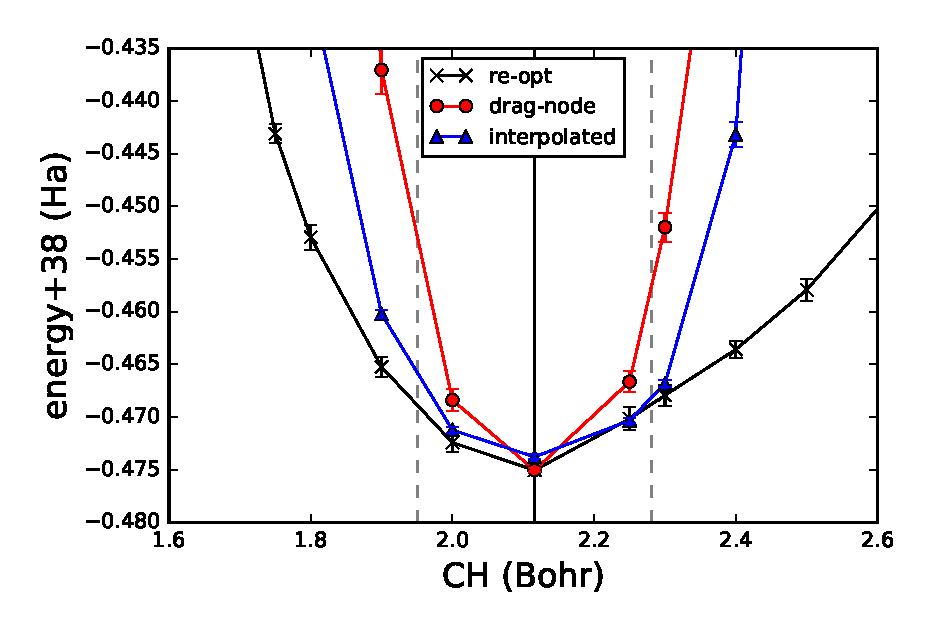
\includegraphics[scale=0.5]{CH-cold}
\caption{Clamped-ion VMC total energy as a function of C-H separation using a hierarchy of wave functions. The dotted lines mark the FWHM of the distribution of C-H separation. \label{fig:ch-cold}}
\end{figure}

\section{Results and Discussion}

In our previous study, wave functions of the form Eq.~\eqref{eqn:wfs2} were used to simulate several different molecular systems~\cite{Yang2015}.  To determine the nonadiabatic energy of each system, we partitioned the energy of our systems into different components, which includes the clamped-ion energies, the zero point energy (ZPE) and the diagonal Born-Oppenheimer energy (DBOC).   Everything that remained we consider to be the nonadiabatic energy.   Using standard quantum chemistry tools all of the above terms can be calculated or approximated to high accuracy with the exception of the nonadiabatic energy.  As a result the nonadiabatic energy is a quantity that has not been theoretically calculated for many systems. It was found in general that the nonadiabatic energy made up less than 0.1~mHa when considering the energy differences between clamped-ion simulations and the full simulation of the electron-ion Hamiltonian.   However, in the case of BH and CH the nonadiabatic effects were  significantly larger than 0.1~mHa.   %Our nonadiabatic energy was over 1~mHa for the CH atom, which is quite large in comparison to all the other systems we consider, and was larger than what was expected from experiment.  However there was only one experimental result and we wanted to consider this calculation in more depth due to the nature of the fixed-node approximation in estimating nonadiabatic effects.

Our new results with the improved wave functions can be see in Table~\ref{tab:energy}.  Due to the variational property of FN-DMC, it is evident that these results are improved energy over the previous best results for the CH molecule, which is not unexpected given the differences between the interpolated wave function and the dragged-node wave function as seen in Fig.~\ref{fig:ch-cold}. Our previous results showed a nonadiabatic energy of roughly 2~mHa. Our new results show a nonadiabatic energy of roughly 1~mHa, which can be seen for the most accurate results in Table~\ref{tab:energy}.  This is not unexpected, as when a system has moderate non-adiabatic energy, more effort is needed in generating accurate wave functions.  Improving the wave functions will lower the estimate of the non-adiabatic energy, but not all the way.  This is what we see for CH, as the non-adiabatic energy is still  relatively large in comparison to other systems.  We note that this is still not a definitive estimate of the nonadiabatic energy, but it is likely the best estimate ever calculated for this system.

We also noticed interesting behavior that results from improving the quality of the electron nodes.  We performed clamped-ion (static) and fully nonadiabatic (dynamic) calculations using different truncations levels for the determinant expansion. FN-DMC energy and variance for the various calculations are shown in Table~\ref{tab:energy}. As we include more determinants in our wave function, both energy and variance of the static calculation decrease. %This confirms that we have better variational wave functions by including more determinants. 
The energy and variance of the dynamic run with determinant coefficient interpolation is always improved  over the wave function without interpolation.  A comparison between the dynamic runs with and without interpolation also shows that coefficient interpolation becomes more important for larger determinant expansion.

\begin{table}[h]
\begin{tabular}{llll}
\hline\hline
$N_{CSF}$ & Energy (Ha) & Variance (Ha$^2$) & method \\
\hline
17   & -38.4709(1) &  0.3130(5) &    static \\
17   & -38.4622(2) &  0.3169(3) &   drag \\
17   & -38.4621(2) &  0.3173(3) &  interp. \\
251  & -38.4770(1)&  0.2489(3) &    static \\
251  & -38.4667(1) &  0.334(2)~  &   drag \\
251  & -38.4679(1) &  0.2713(7) &  interp. \\
1417 & -38.4781(1) &  0.2300(4) &    static \\
1417 & -38.4676(1) &  0.334(5)~  &   drag \\
1417 & -38.4687(2) &  0.267(7)~  &  interp. \\
\hline\hline
\end{tabular}
\caption{DMC energy and variance with static ions, dynamic ions with dragged-node (``drag'') and dynamic ions with determinant coefficient interpolation (``interp.'').\label{tab:energy}}
\end{table}

In Fig.~\ref{fig:ch-interp} we show the various contributions to the difference between the static and dynamic ground-state energies as calculated from Table~\ref{tab:energy}. Due to the difference in energy scales for the different quantities of interest, we only plot the diagonal Born-Oppenheimer energy and the nonadiabatic energy.   The estimated zero-point energy for CH is  6.438 mHa~\cite{Feller_Corrections}. The diagonal Born-Oppenheimer correction is estimated to be 2.11 mHa~\cite{Yang2015}. Our best result is represented as the right-most bar in Fig.~\ref{fig:ch-interp}.  This run includes the most number of determinants and takes advantage of coefficient interpolation. It is clear that there was significant artificial contribution to the nonadiabatic energy of CH from the dragged-node approximation. However, the fact that CH is the only molecule where dragged-node approximation fails suggests the nodal structure of its wave function has more complex dependence on the ion configuration than the rest of the molecules under consideration.

Comparing all bar plots in Fig.~\ref{fig:ch-interp} reveals that the nonadiabatic energy is only captured with a large determinant expansion. In addition, the dragged-node approximation does not fail for the smallest determinant expansion we tested. One possible explanation is that the intricacies of the ion-dependence of the nodal surface comes from the inclusion of highly excited determinants. While giving rise to a better electronic wave function at any fixed ion position, these intricacies caused the drag-node approximation to fail and lead to an artificial contribution to the nonadaibatic energy in our original calculation.

\begin{figure}[h]
%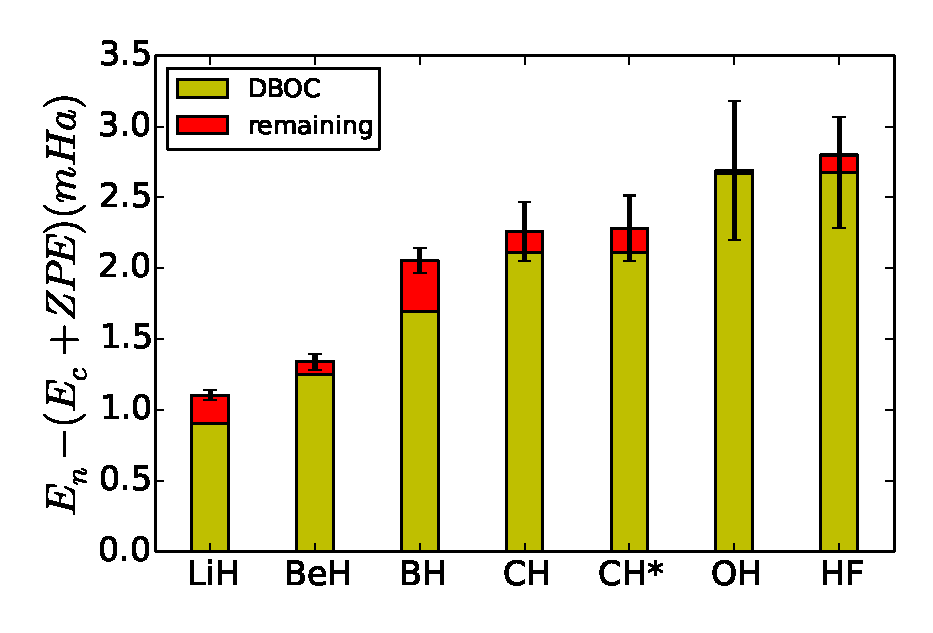
\includegraphics[scale=0.5]{35}
%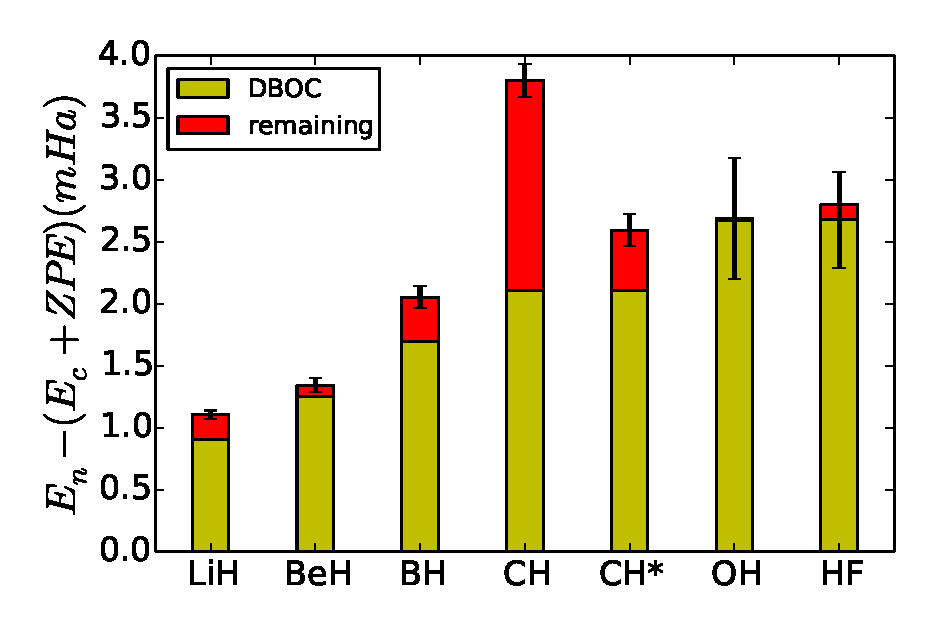
\includegraphics[scale=0.5]{723}
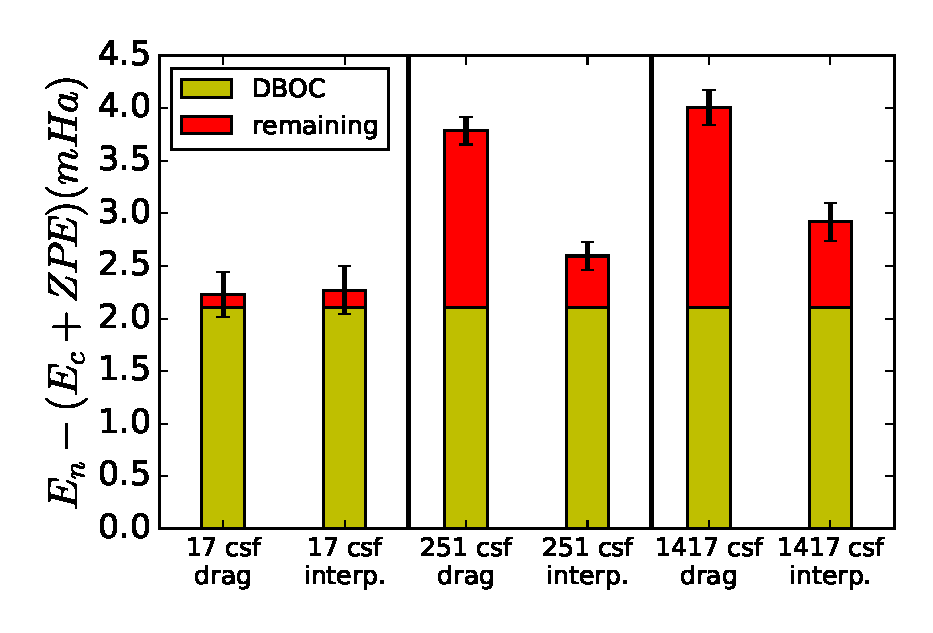
\includegraphics[scale=0.5]{ch-only}
\caption{Nonadiabatic energy of CH with and without determinant coefficient interpolation. Solid verticle lines separate calculations with different number of CSFs. ``interp.'' denotes that the determinant coefficients depend on C-H separation through linear interpolation. \label{fig:ch-interp} }
\end{figure}

\begin{figure}[h]
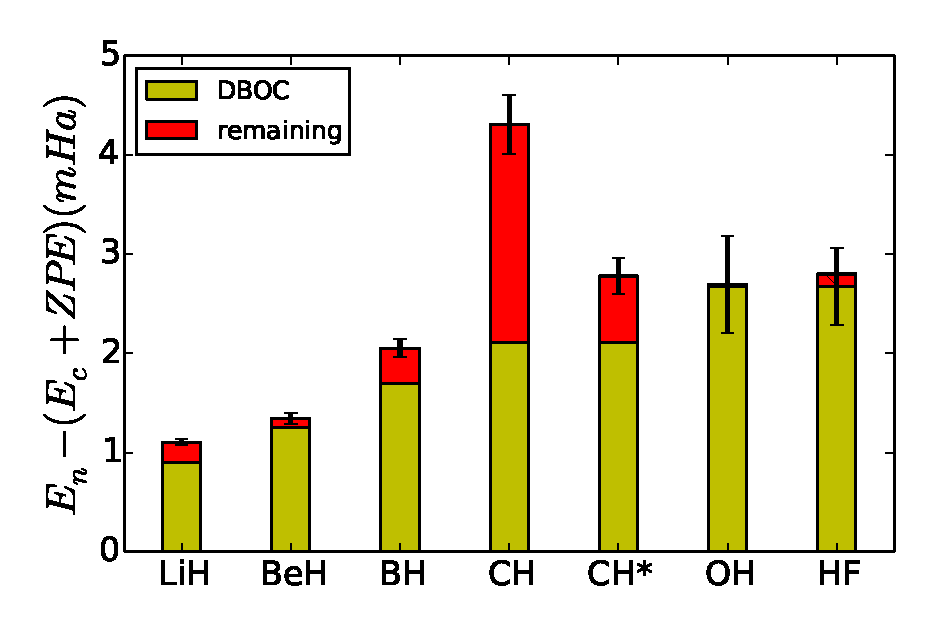
\includegraphics[scale=0.5]{4738}
\caption{Nonadiabatic energy of diatomic molecules explored in Ref.~\cite{Yang2015}. The best (1417 CSFs) result for CH with determinant coefficient interpolation is shown with *. }
\end{figure}

\begin{comment}
\begin{figure}[h]
\includegraphics[scale=0.55]{two-point-fit}
\caption{Two-point fit for the determinant coefficients.\label{fig:two-point-fit}}
\end{figure}

\begin{figure}[h]
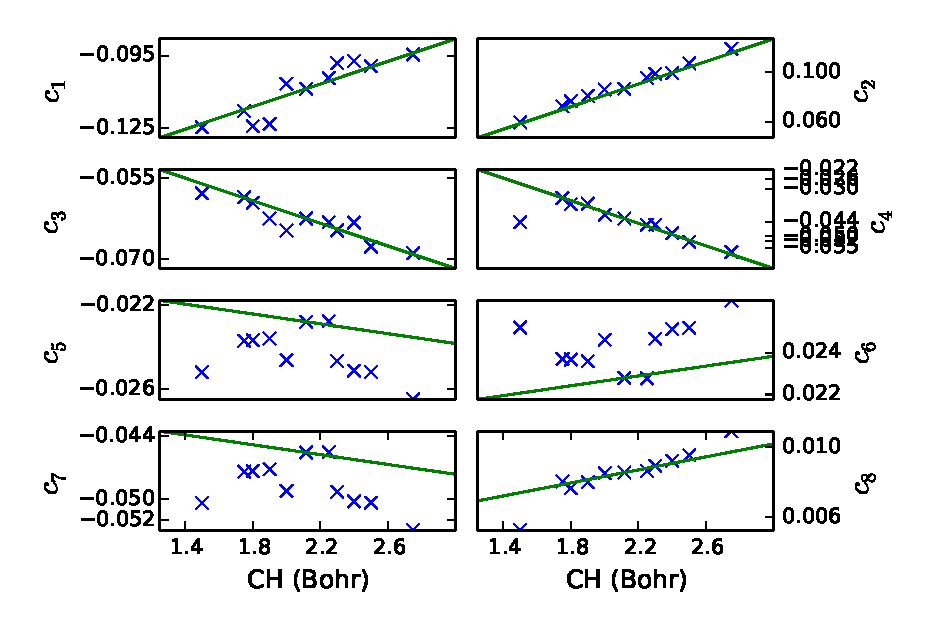
\includegraphics[scale=0.55]{one-point-fit}
\caption{One-point fit for the determinant coefficients.\label{fig:one-point-fit}}
\end{figure}

\begin{figure}[h]
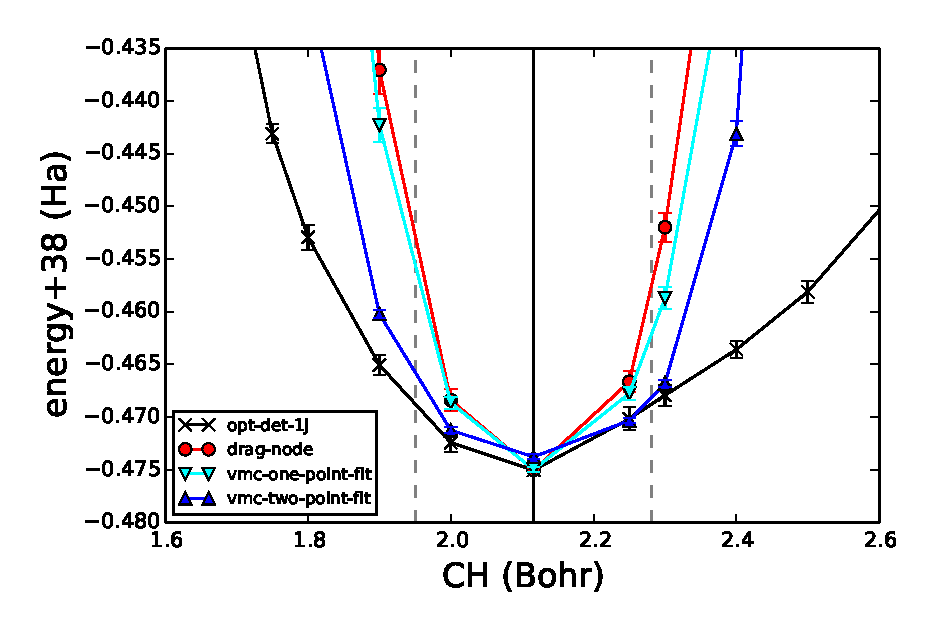
\includegraphics[scale=0.5]{CH-fit-energy}
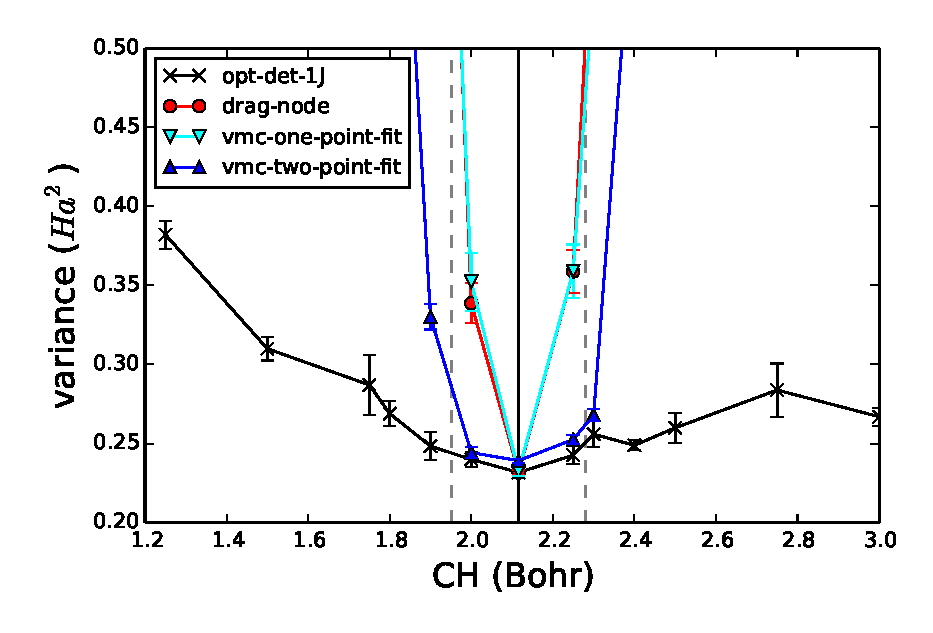
\includegraphics[scale=0.5]{CH-fit-variance}
\caption{Quality of the various forms wave function, quantified by energy and variance at the variational level. \label{fig:wf quality} }
\end{figure}
\end{comment}


\section{Conclusion}

In this work, we demonstrated that for diatomic systems, there are ways of generating wave functions beyond what has been done in previous quantum Monte Carlo work.  These wave functions are generated from highly accurate static quantum chemistry techniques, from which nodes are derived that are better than those of the dragged-node approximation.  We have been explicitly interested in the CH molecule, due to our previous results that show some what large nonadiabatic energy, and in this work we improve upon our estimate of this energy.  Further calculations are possible to improve our results here, such as release node calculations, however, real progress for larger systems will require even more clever scheme to improve wave functions.   This is however is a further step to improve the accuracy of nonadiabatic simulations to start approaching the accuracy needed to compare to spectroscopic results and predictions for the peaks in the ISM.


\section{Acknowledgment}
NT was supported through the Scientific Discovery through Advanced Computing (SciDAC) program funded by the U.S. Department of Energy, Office of Science, Advanced Scientific Computing
Research, and Basic Energy Sciences.  This work used the Extreme Science and Engineering Discovery Environment (XSEDE), which is supported by National Science Foundation grant number ACI-1053575.   DC was supported through  DOE grant DE-NA0001789. Y.Y. acknowledges the computational science and engineering (CSE) fellowship from University of Illinois Urbana-Champaign. S.H.S. acknowledges support by the National Science Foundation under CHE-13-61293. We used resources of the Oak Ridge Leadership Computing Facility (OLCF) at the Oak Ridge National Laboratory, which is supported by the Office of Science of the U.S. Department of Energy under Contract No. DE-AC05-00OR22725.

\bibliography{ref}
\end{document}
